% -*- latex -*-
%%%%%%%%%%%%%%%%%%%%%%%%%%%%%%%%%%%%%%%%%%%%%%%%%%%%%%%%%%%%%%%%
%%%%%%%%%%%%%%%%%%%%%%%%%%%%%%%%%%%%%%%%%%%%%%%%%%%%%%%%%%%%%%%%
%%%%
%%%% This text file is part of the lecture slides for
%%%% `Parallel Computing'
%%%% by Victor Eijkhout, copyright 2012-2021
%%%%
%%%% Graph-slides.tex : slides about MPI graph topologies
%%%%
%%%%%%%%%%%%%%%%%%%%%%%%%%%%%%%%%%%%%%%%%%%%%%%%%%%%%%%%%%%%%%%%
%%%%%%%%%%%%%%%%%%%%%%%%%%%%%%%%%%%%%%%%%%%%%%%%%%%%%%%%%%%%%%%%

\begin{numberedframe}{Overview}
  This section discusses graph topologies.

  Commands learned:
  \begin{itemize}
  \item \indexmpishow{MPI_Dist_graph_create}, \indexmpishow{MPI_DIST_GRAPH},
    \indexmpishow{MPI_Dist_graph_neighbors_count}
  \item \indexmpishow{MPI_Neighbor_allgather} and such
  \end{itemize}
\end{numberedframe}

\begin{numberedframe}{Process topologies}
  \begin{itemize}
  \item Processes don't communicate at random
  \item Example: Cartesian grid, each process 4 (or so) neighbors
  \item Express operations in terms of topology
  \item Elegance of expression
  \end{itemize}
\end{numberedframe}

\begin{numberedframe}{Process reordering}
  \begin{itemize}
  \item Consecutive process numbering often the best:\\
    divide array by chunks
  \item Not optimal for grids or general graphs:
  \item MPI is allowed to renumbering ranks
  \item Graph topology gives information from which to deduce
    renumbering
  \end{itemize}
\end{numberedframe}

\begin{numberedframe}{MPI-1 topology}
  \begin{itemize}
  \item Cartesian topology
  \item Graph topology, globally specified.\\
    Not exactly scalable!
  \end{itemize}
\end{numberedframe}

\begin{numberedframe}{MPI-3 topology}
  \begin{itemize}
  \item Graph topologies locally specified: scalable!
  \item Neighborhood collectives:\\
    expression close to the algorith.
  \end{itemize}
\end{numberedframe}

\begin{numberedframe}{Example: 5-point stencil}
  Neighbor exchange,
  spelled out:
  \begin{itemize}
  \item Each process communicates down/right/up/left
  \item Send and receive at the same time.
  \item Can optimally be done in four steps
  \end{itemize}
\end{numberedframe}

\begin{numberedframe}{Step 1}
  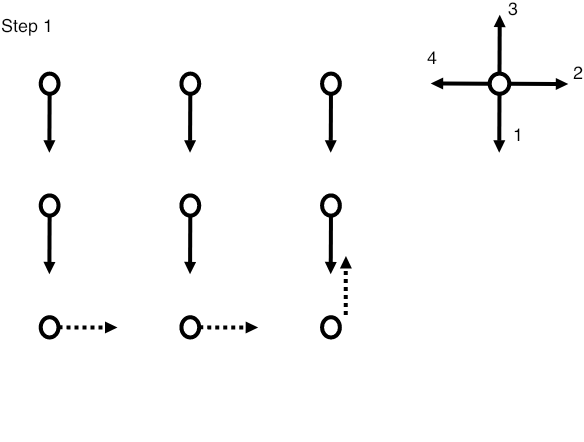
\includegraphics[scale=.4]{gropptiming1}
\end{numberedframe}

\begin{numberedframe}{Step 2}
  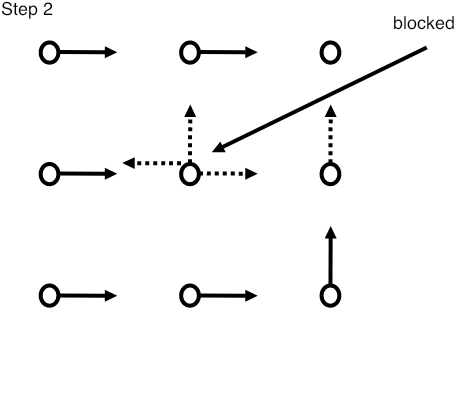
\includegraphics[scale=.4]{gropptiming2}

  The middle node is blocked because all its targets
  are already receiving\\
  or a channel is occupied:\\
  one missed turn
\end{numberedframe}

\begin{numberedframe}{Neighborhood collective}
  \label{fig:graphcollective}
  This is really a `local gather':\\
  each node does a gather from its neighbors in whatever order.\\
  \indexmpishow{MPI_Neighbor_allgather}

  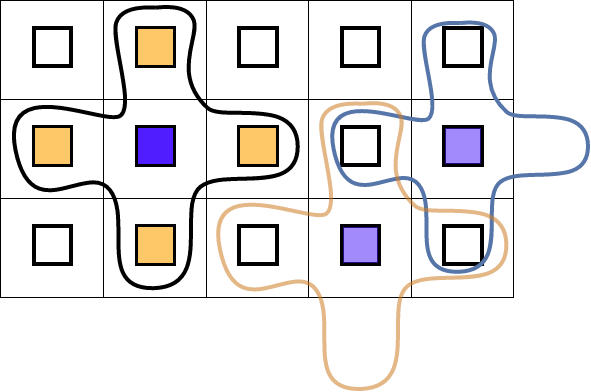
\includegraphics[scale=.5]{graphcollective}

  Distributed graph topology where each
  node has four neighbors
\end{numberedframe}

\begin{numberedframe}{Why neighborhood collectives?}
  \begin{itemize}
  \item Using \indexmpishow{MPI_Isend}~/ \indexmpishow{MPI_Irecv} is like spelling out a collective;
  \item Collectives can use pipelining as opposed to sending  a whole
    buffer;
  \item Collectives can use spanning trees as opposed to direct connections.
  \end{itemize}
\end{numberedframe}

\begin{numberedframe}{Create graph topology}
\lstset{language=C}
\begin{lstlisting}
int MPI_Dist_graph_create
   (MPI_Comm comm_old, int nsources, const int sources[],
    const int degrees[], const int destinations[], 
    const int weights[], MPI_Info info, int reorder,
    MPI_Comm *comm_dist_graph)
\end{lstlisting}
\begin{itemize}
\item \lstinline{nsources} how many source nodes described? (Usually~1)
\item \lstinline{sources} the processes being described (Usually
  \indexmpishow{MPI_Comm_rank} value)
\item \lstinline{degrees} how many processes to send to
\item \lstinline{destinations} their ranks
\item \lstinline{weights}: usually set to \indexmpishow{MPI_UNWEIGHTED}.
\item \lstinline{info}: \indexmpishow{MPI_INFO_NULL} will do
\item \lstinline{reorder}: 1~if dynamically reorder processes
\end{itemize}
\end{numberedframe}

\begin{numberedframe}{Neighborhood collectives}
\begin{lstlisting}
int MPI_Neighbor_allgather
   (const void *sendbuf, int sendcount,MPI_Datatype sendtype,
    void *recvbuf, int recvcount, MPI_Datatype recvtype,
    MPI_Comm comm)
\end{lstlisting}
Like an ordinary \indexmpishow{MPI_Allgather}, but\\
the receive buffer has a length \lstinline{degree}.
\end{numberedframe}

\begin{numberedframe}{Neighbor querying}
  \label{sl:graph-neighbors}
  After \indexmpishow{MPI_Neighbor_allgather} data in the buffer
  is \emph{not} in normal rank order.
  \begin{itemize}
  \item \indexmpishow{MPI_Dist_graph_neighbors_count} gives actual number of neighbors.\\
    (Why do you need this?)
  \item 
    \indexmpidef{MPI_Dist_graph_neighbors} lists neighbor numbers.
  \end{itemize}
\end{numberedframe}

\protoslide{MPI_Dist_graph_neighbors}

\begin{exerciseframe}[rightgraph]
  \hyperlink{exserialsend}{\beamergotobutton{Earlier rightsend exercise}}

  \input ex:rightgraph
\end{exerciseframe}

\begin{numberedframe}{Inspiring picture for the previous exercise}
  \label{fig:rightgraph}

  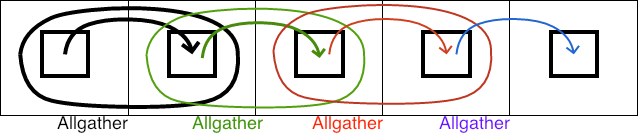
\includegraphics[scale=.5]{rightgraph}

  Solving the right-send exercise with neighborhood
  collectives
\end{numberedframe}

\begin{numberedframe}{Hints for the previous exercise}
  Two approaches:
  \begin{enumerate}
  \item Declare just one source: the previous process. Do this! Or:
  \item Declare two sources: the previous and yourself.
    In that case bear in mind slide~\ref{sl:graph-neighbors}.
  \end{enumerate}
\end{numberedframe}

\endinput

\begin{numberedframe}{}
\end{numberedframe}

